% !TeX root = ./PhDThesis.tex

\chapter{Experimental setup}

The rate of background gas collisions with the ion chain is one of the scaling challenges in an ion-trapped system. Such collisions may destroy the qubit's information and result in the loss of the whole chain. Thus, it is essential to construct an extreme high vacuum (XHV) environment to reduce the vacuum system's background gas pressure.



\section{The cryostat}

The cryostat is the key equipment of the cryogenic trapped ion system. We need to pay attention to some key technical indicators when choosing the model of the cryostat, designing the internal support structure and the assembly structure of the trap-related components. The most critical technical indicators are cooling capacity and vibration. Low temperature is the advantage of the cryogenic trap over the room-temperature trap. We can achieve low pressure by cryo-pumping to reduce the collision rate of trapped ions with residual background gas, thereby increasing the lifetime of trapped ions. The price of cryo-pumping is additional vibration, however, the vibration can be reduced to a degree that does not affect quantum gate fidelity. In experiments, we often use these two parameters to characterize the cooling capacity. One is the lowest temperature that the system can reach when the cryogenic trap is not temperature stabilized, and the other is the heating power at the sample mount when the temperature of the cryogenic trap is stabilized above the liquid helium temperature zone and the vibration caused by liquid helium is reduced to a certain range. Another key technical indicator of the cryostat is the long-term stability at the sample, including changes in displacement and background electric field. This will affect the calibration period of the ion trap experiment. Calibration that is too frequent indicates a lack of robustness in the experiment system.

There are several different types of cryostats on the market. One of these is the flow cryostat, which has lower cryocooler vibration noise but requires constant replenishment of cold liquid coolant, which is expensive and time-consuming. In contrast, the cryogenic trapped ion system in our lab uses a closed-loop Gifford-McMahon cryostat. This type of cryostat uses closed-cycle helium gas as operation material in cooling cycle and does not require constant refilling of the coolant. It is very convenient to use and cheap to maintain as it only needs external electric supply.
One of the advantages of this closed-loop cryostat is that it has a vibration isolation system (VIS). The vibrating cold finger is mechanically separated from the main vacuum by a helium-filled exchange gas region at a pressure 0.03 bar above atmospheric. The vibration isolation system is the only mechanical coupling between the cold head and the main vacuum apparatus which is mounted on an optical breadboard. In the vibration isolation system region, it is sealed with a helium-confined rubber bellows. The helium gas serves as the thermal link between the cold finger and the sample mount where the ion trap is mounted. Another advantage of this closed-cycle cryostat is that its structure is relatively simple, and we can increase cooling capacity and reduce vibration through optimized design, because it is difficult to optimize each parameter independently in a complex system.

\begin{table}
    \centering
    \caption{Refrigeration capacity (typical).}
    \begin{tabular}{p{0.2\linewidth}p{0.3\linewidth}p{0.3\linewidth}}
        \toprule
                     & RDK-408D2                 & RDK-415D2                 \\
        \midrule
        First stage  & 40 Watts @ 43 (50Hz)      & 35 Watts @ 50K (50Hz)     \\
                     & 50 Watts @ 43 (60Hz)      & 45 Watts @ 50K (60Hz)     \\
        Second stage & 1.0 Watt @ 4.2K (50/60Hz) & 1.5 Watt @ 4.2K (50/60Hz) \\
        \bottomrule
    \end{tabular}
    \label{tab:refrigeration_capacity}
\end{table}

The cryostat is model SHI-4XG-15-UHV, designed and manufactured by Janis Inc. In order to reduce vibration, we provide some design suggestions. The cryostat consists of a cold head, an exchange gas space and a vacuum chamber.
The cold head is powered by a helium compressor. The models of cold head and helium compressor are RDK-415D2 and F70-H produced by Sumitomo Corporation of Japan. The cold head features two stages with different refrigeration capacity: the 40 K stage has $\sim$ 35 W, and the 4 K stage has 1.5 W, as shown in Table~\ref{tab:refrigeration_capacity}. The cold head must be fixed near the vacuum chamber, but there are only three interfaces of the cold head: the power supply, the supply high-pressure helium tube and the return high-pressure helium tube. Therefore, we placed the helium compressor and water cooler in the grey room of the laboratory to further isolate the source of vibration noise. The single continuous running time of the cold head can exceed 10,000 hours, which is enough for us to carry out long-term experiments.

\begin{figure}
    \centering
    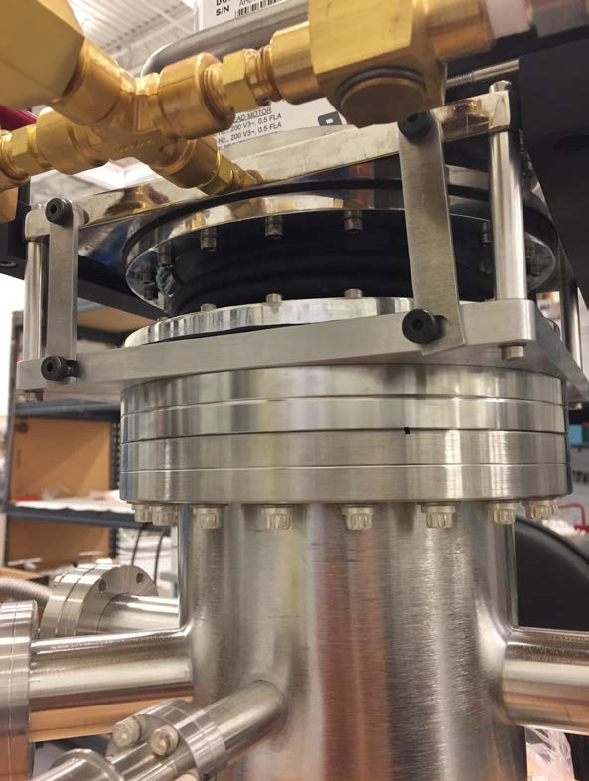
\includegraphics[width=0.5\linewidth]{fig_3_exchange_gas_space.pdf}
    \caption{Exchange gas space.}
    \label{fig:exchange_gas_space}
\end{figure}

The exchange gas space, as shown in Fig~\ref{fig:exchange_gas_space}, is mainly composed of rubber bellow, helium pressure gauge and some helium valves, the top and bottom are respectively connected to the cold head and the vacuum chamber. The role of bellow is to reduce the vibration generated by the cold head and directly transmitted to the vacuum chamber, because rubber is more elastic than stainless steel. I think it is worth trying to replace the rubber bellow with a stainless-steel sheet that has been bent many times, because using a rubber bellow may cause leakage in the long-term operation of the system. Leakage of rubber bellow may come from three aspects. Firstly, the rubber material will deteriorate after a long-time use, our system has a leakage problem after about 2 years of operation, which is manifested as water inside the exchange gas space after the process of cooling down and warming up. Secondly, the rubber bellow is prone to defects during machining, we contacted our supplier to process a new rubber bellow after we found the leakage problem, and found that some of the rubber bellow had defects on the surface during many attempts. Finally, the sealing method of rubber bellow is worse than that of stainless steel, our cryostat uses o-ring to seal rubber bellow. We tried to have the supplier process different rubber bellow to test the leakage, such as testing different materials and thickness of rubber bellow, in some poor cases after a single cooling and reheating process will appear leakage, we finally used silicone rubber bellow and the thickness is twice the original and no leakage has been found so far.



\section{Cryogenic and UHV system}

\begin{figure}
    \centering
    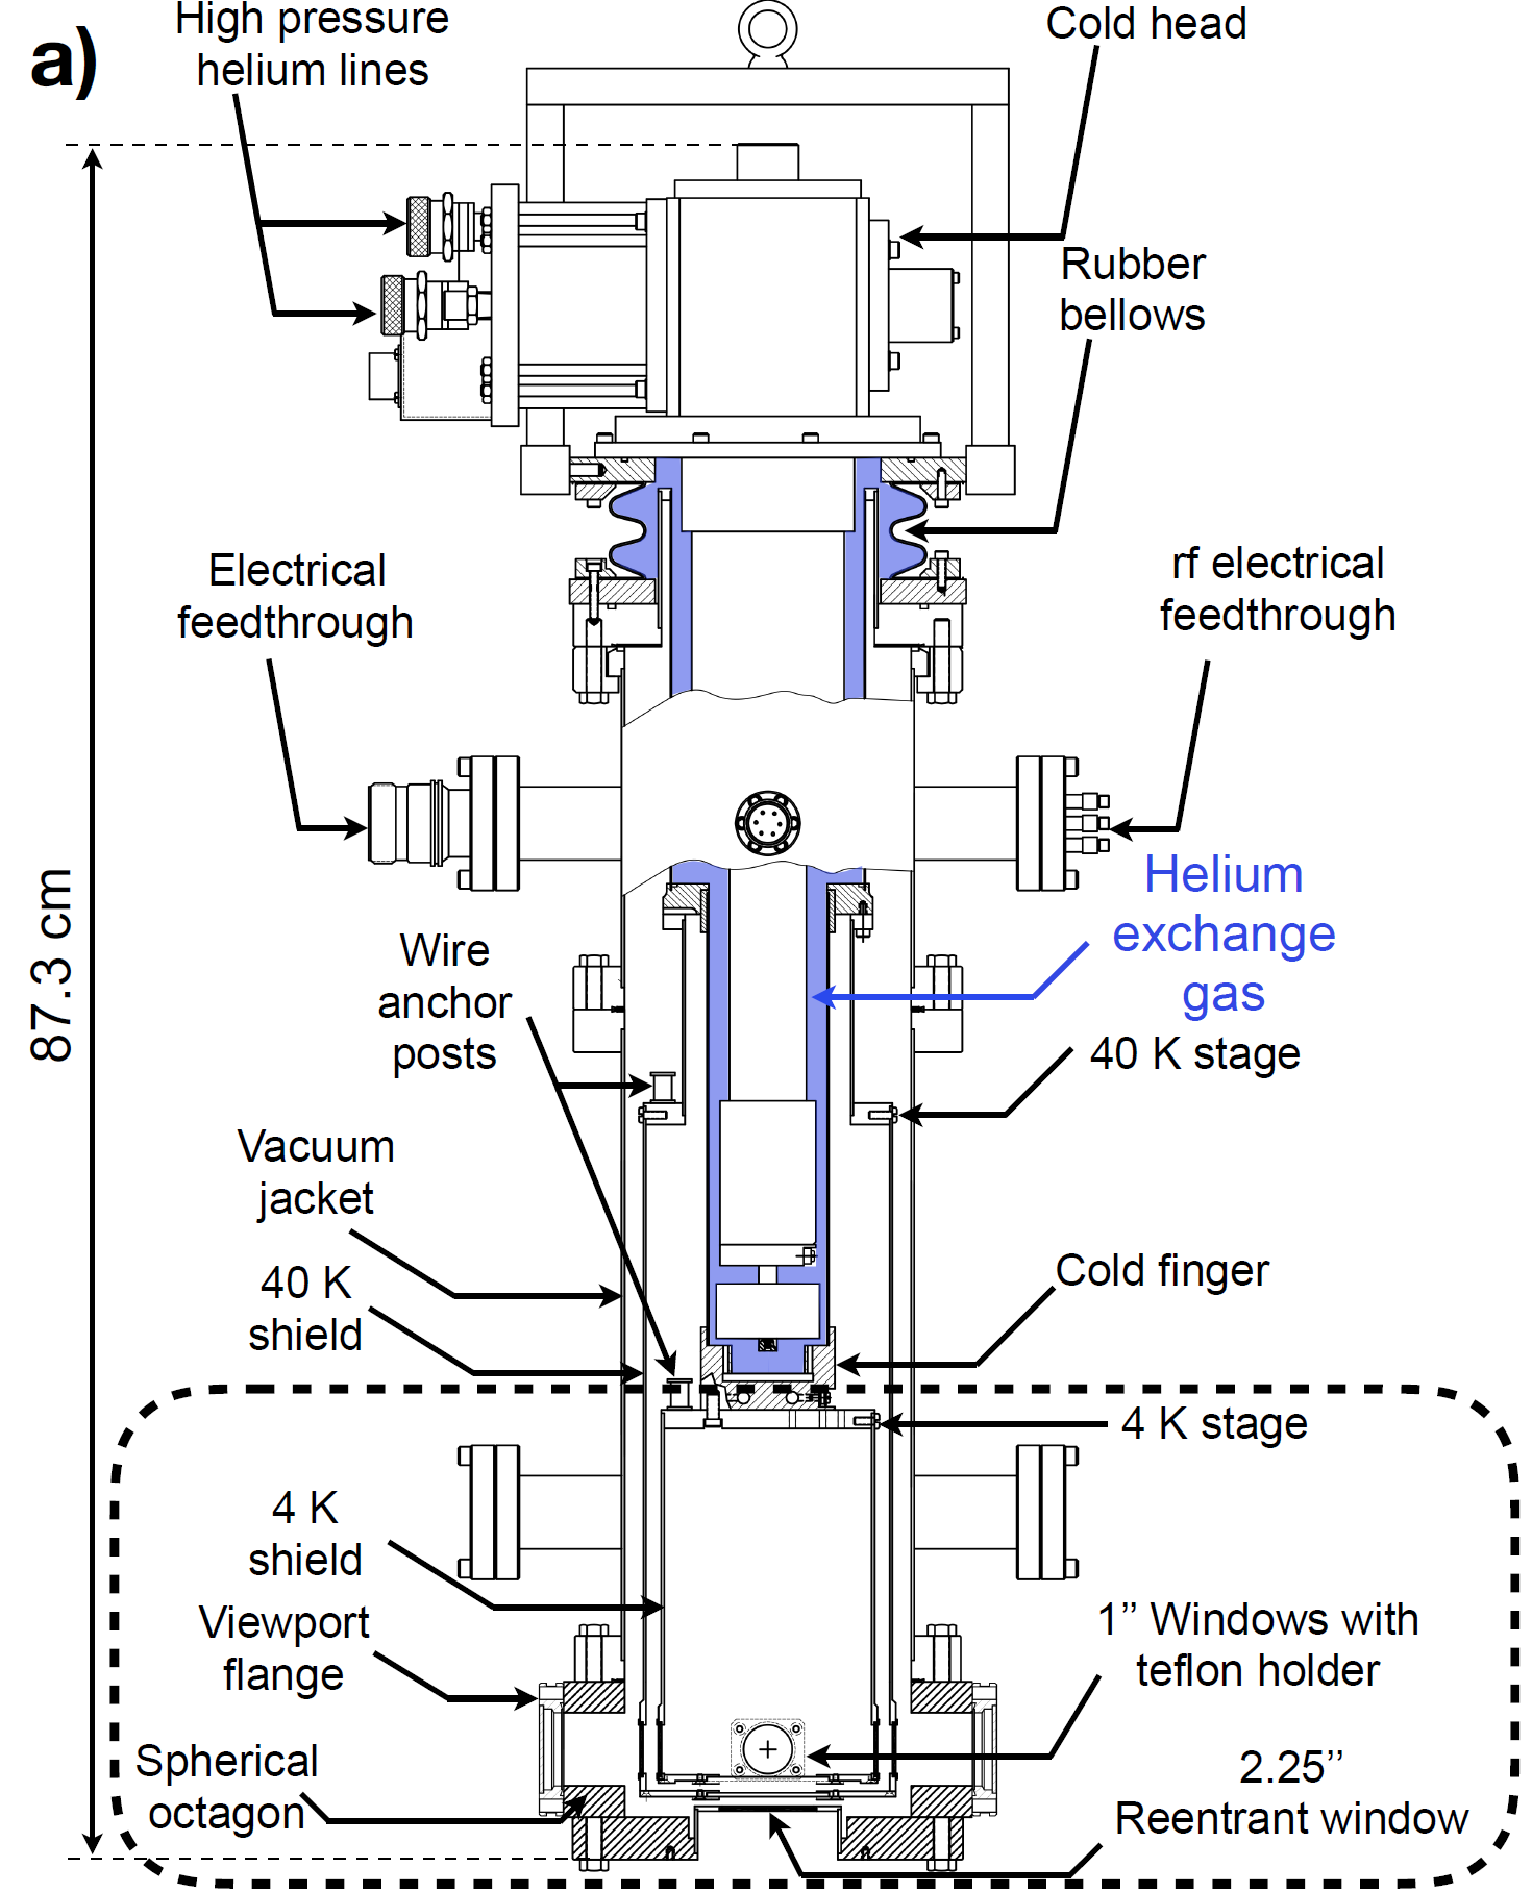
\includegraphics[width=0.7\linewidth]{fig_3_cryostat_a.pdf}
    \caption{The side section view of the Gilford-McMahon cryostat.}
    \label{fig:cryostat_a}
\end{figure}

The vacuum chamber resembles a cylinder with a diameter of about 200 mm and a height of about 600 mm. Externally, the upper part of the vacuum chamber has some feedthroughs connecting the electrical equipment to the vacuum equipment, and the lower part is a spherical octagon. The top of the vacuum chamber is in contact with the exchange gas space, and the bottom is the re-entrant window. In our experiments, we used a total of three electrical feedthroughs, one DC feedthrough to drive the voltage signal to the electrodes of the trap, another DC feedthrough to drive the thermometer and heater in the vacuum chamber, and an RF feedthrough to drive the RF signal to the resonator. Below them, there are a total of three Vacuum feedthroughs, one connected to an ion gauge (Agilent UHV-24P) to monitor the vacuum level in the vacuum chamber, one connected to a NEG-Ion pump (SAES NextTorr Z100) to pump out hydrogen, since hydrogen is the least efficiently cryo-pumped gas, and an angle valve to pump out vacuum during system maintenance. A spherical octagon holds eight 1'' diameter windows to provide optical access in the horizontal plane, the windows are made of UVFS and have different wavelength optical coatings according to the optical path design. We replaced one of the windows along the trap axis with an oven feedthrough, and installed both enriched ${ }^{171} \mathrm{Yb}$ oven and enriched ${ }^{174} \mathrm{Yb}$ oven on it, and finally tested them to work. However, assembly errors during installation may cause the Yb flux cannot enter the trap during ion loading, we can increase the translation degrees of freedom when designing the part to solve this problem. According to our experience, because of the large divergence angle of Yb flux, we just need to be able to see the trap and oven through the opposite window. The re-entrant window located at the bottom of the vacuum chamber has a diameter of 2.25'', below which is the imaging system. The maximum numerical aperture allowed for imaging ions along the vertical direction is 0.5. The Re-entrant window is surrounded by a doughnut-shaped aluminum base placed on an optical breadboard, and the base carries the full weight of the vacuum chamber. We tried to fasten between the upper part of the vacuum chamber and the optical breadboard with an aluminum sloped beam, but it did not reduce the vibration of the trap, indicating that the current support structure is solid enough.

\begin{table}
    \centering
    \caption{List of electrical devices connected to the vacuum chamber.}
    \begin{tabular}{ll}
        \toprule
        Device           & Model                      \\
        \midrule
        ion gauge        & Agilent UHV-24P            \\
        NEG-Ion pump     & AES NextTorr Z100          \\
        DC signal source & Homemade 16-channel AD5791 \\
        RF signal source & Rohde \& Schwarz SMB-100B  \\
        \bottomrule
    \end{tabular}
\end{table}

The main components inside the vacuum chamber are the 40 K shield, the 4 K shield and the sample mount. These two shields are used to shield the ion trap from room temperature blackbody radiation, their material is aluminum, but copper may be a better choice because copper material has a higher thermal conductivity. The bottom of the two shields are eight 1" UVFS windows, which correspond to the spherical octagon and have the same optical coating. The glass is fixed in the groove by the Teflon holder in order to keep the windows from being crushed during the cooling procedure, however, because of the elasticity of Teflon, the positioning accuracy of the windows is poor, which may be the main source of optical aberration. The top of the 40 K shield is in contact with the 40 K stage of the cold head through the helium gas in the exchange gas space, which is usually higher than 40 K, we named it that way just because it is intuitive. The top of the 4 K shield is fixed to the sample mount, which is made of oxygen-free copper with a gold-plated surface to obtain a high thermal conductivity and to prevent oxidation during system maintenance. The sample mount and the 4 K stage of the cold head are separated by a heat exchanger and cryogenic helium gas. The 4 K stage can reach temperatures below 4 K, and the heat exchanger is composed of a series of concentric circular oxygen-free copper sheets, which are designed to increase the cooling capacity at the sample mount. However, if the position between a pair of heat exchangers is shifted during operation and touches each other, it can introduce large vibrations to the sample mount, for example when floating the optical table.

\begin{figure}
    \centering
    \subcaptionbox{The top view of ion trap and vacuum chamber.\label{fig:cryostat_b}}
    {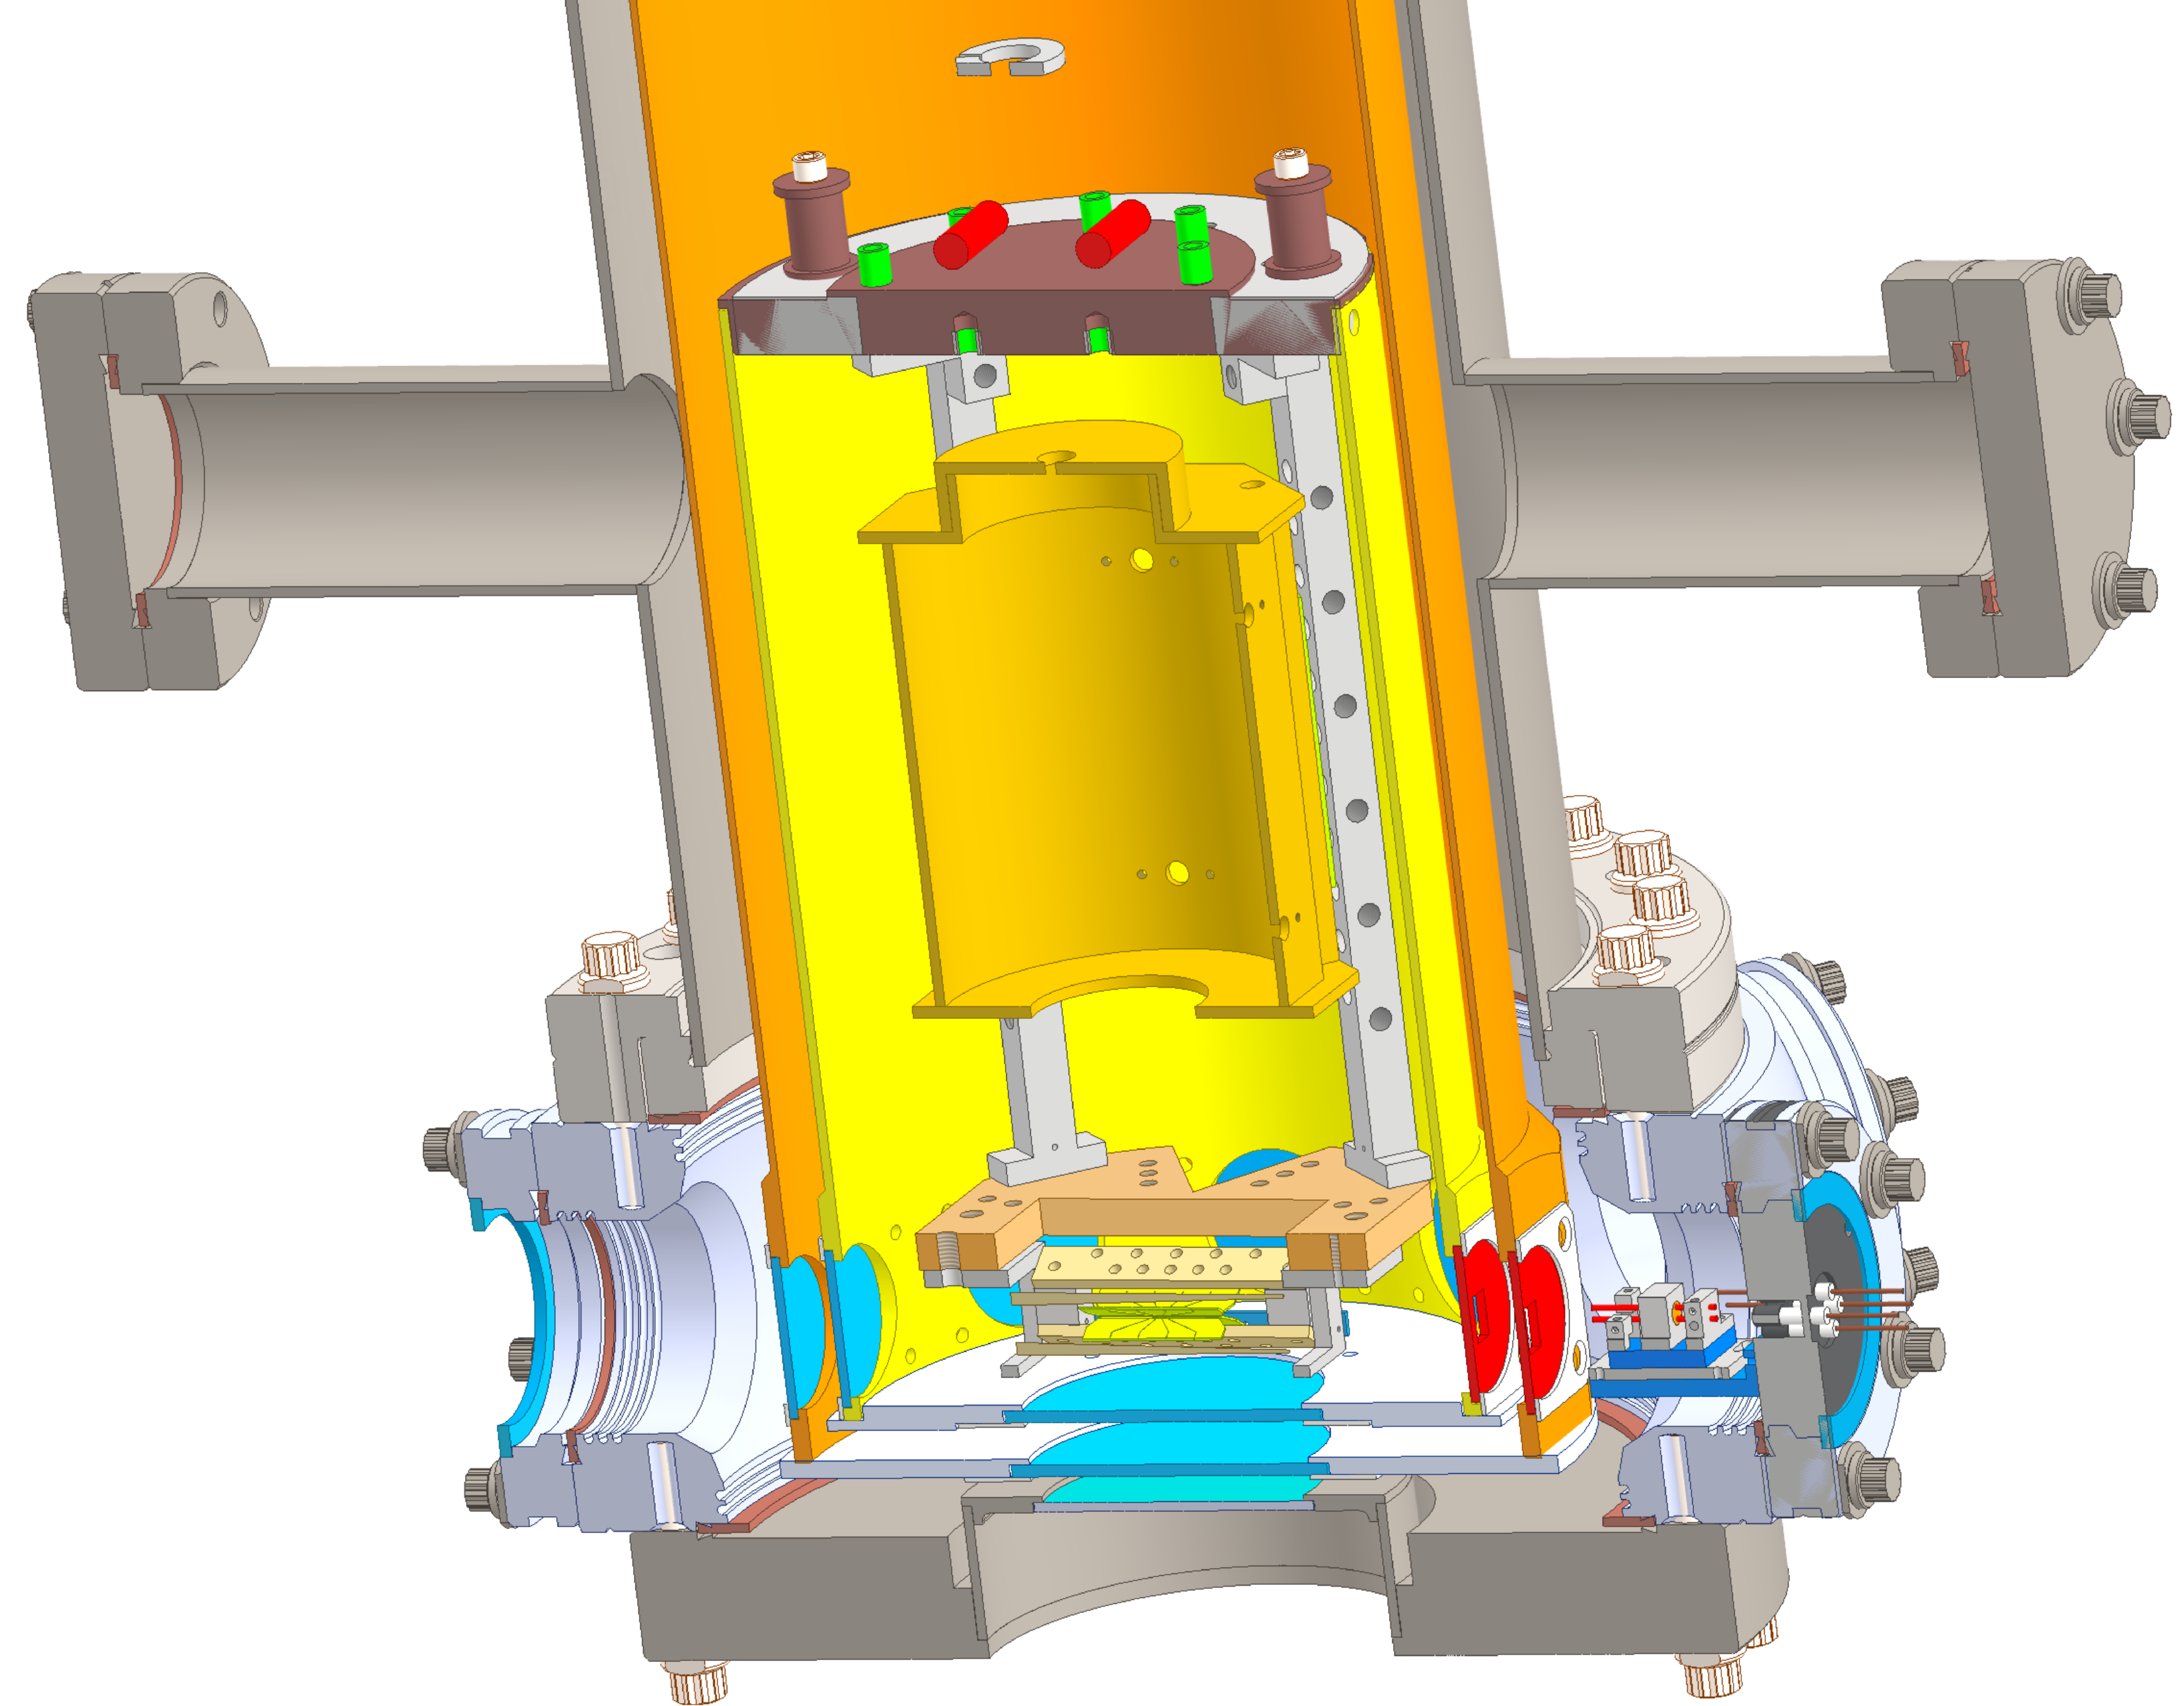
\includegraphics[width=0.4\linewidth]{fig_3_cryostat_b.pdf}}
    \subcaptionbox{The oblique view of ion trap and vacuum chamber.\label{fig:cryostat_c}}
    {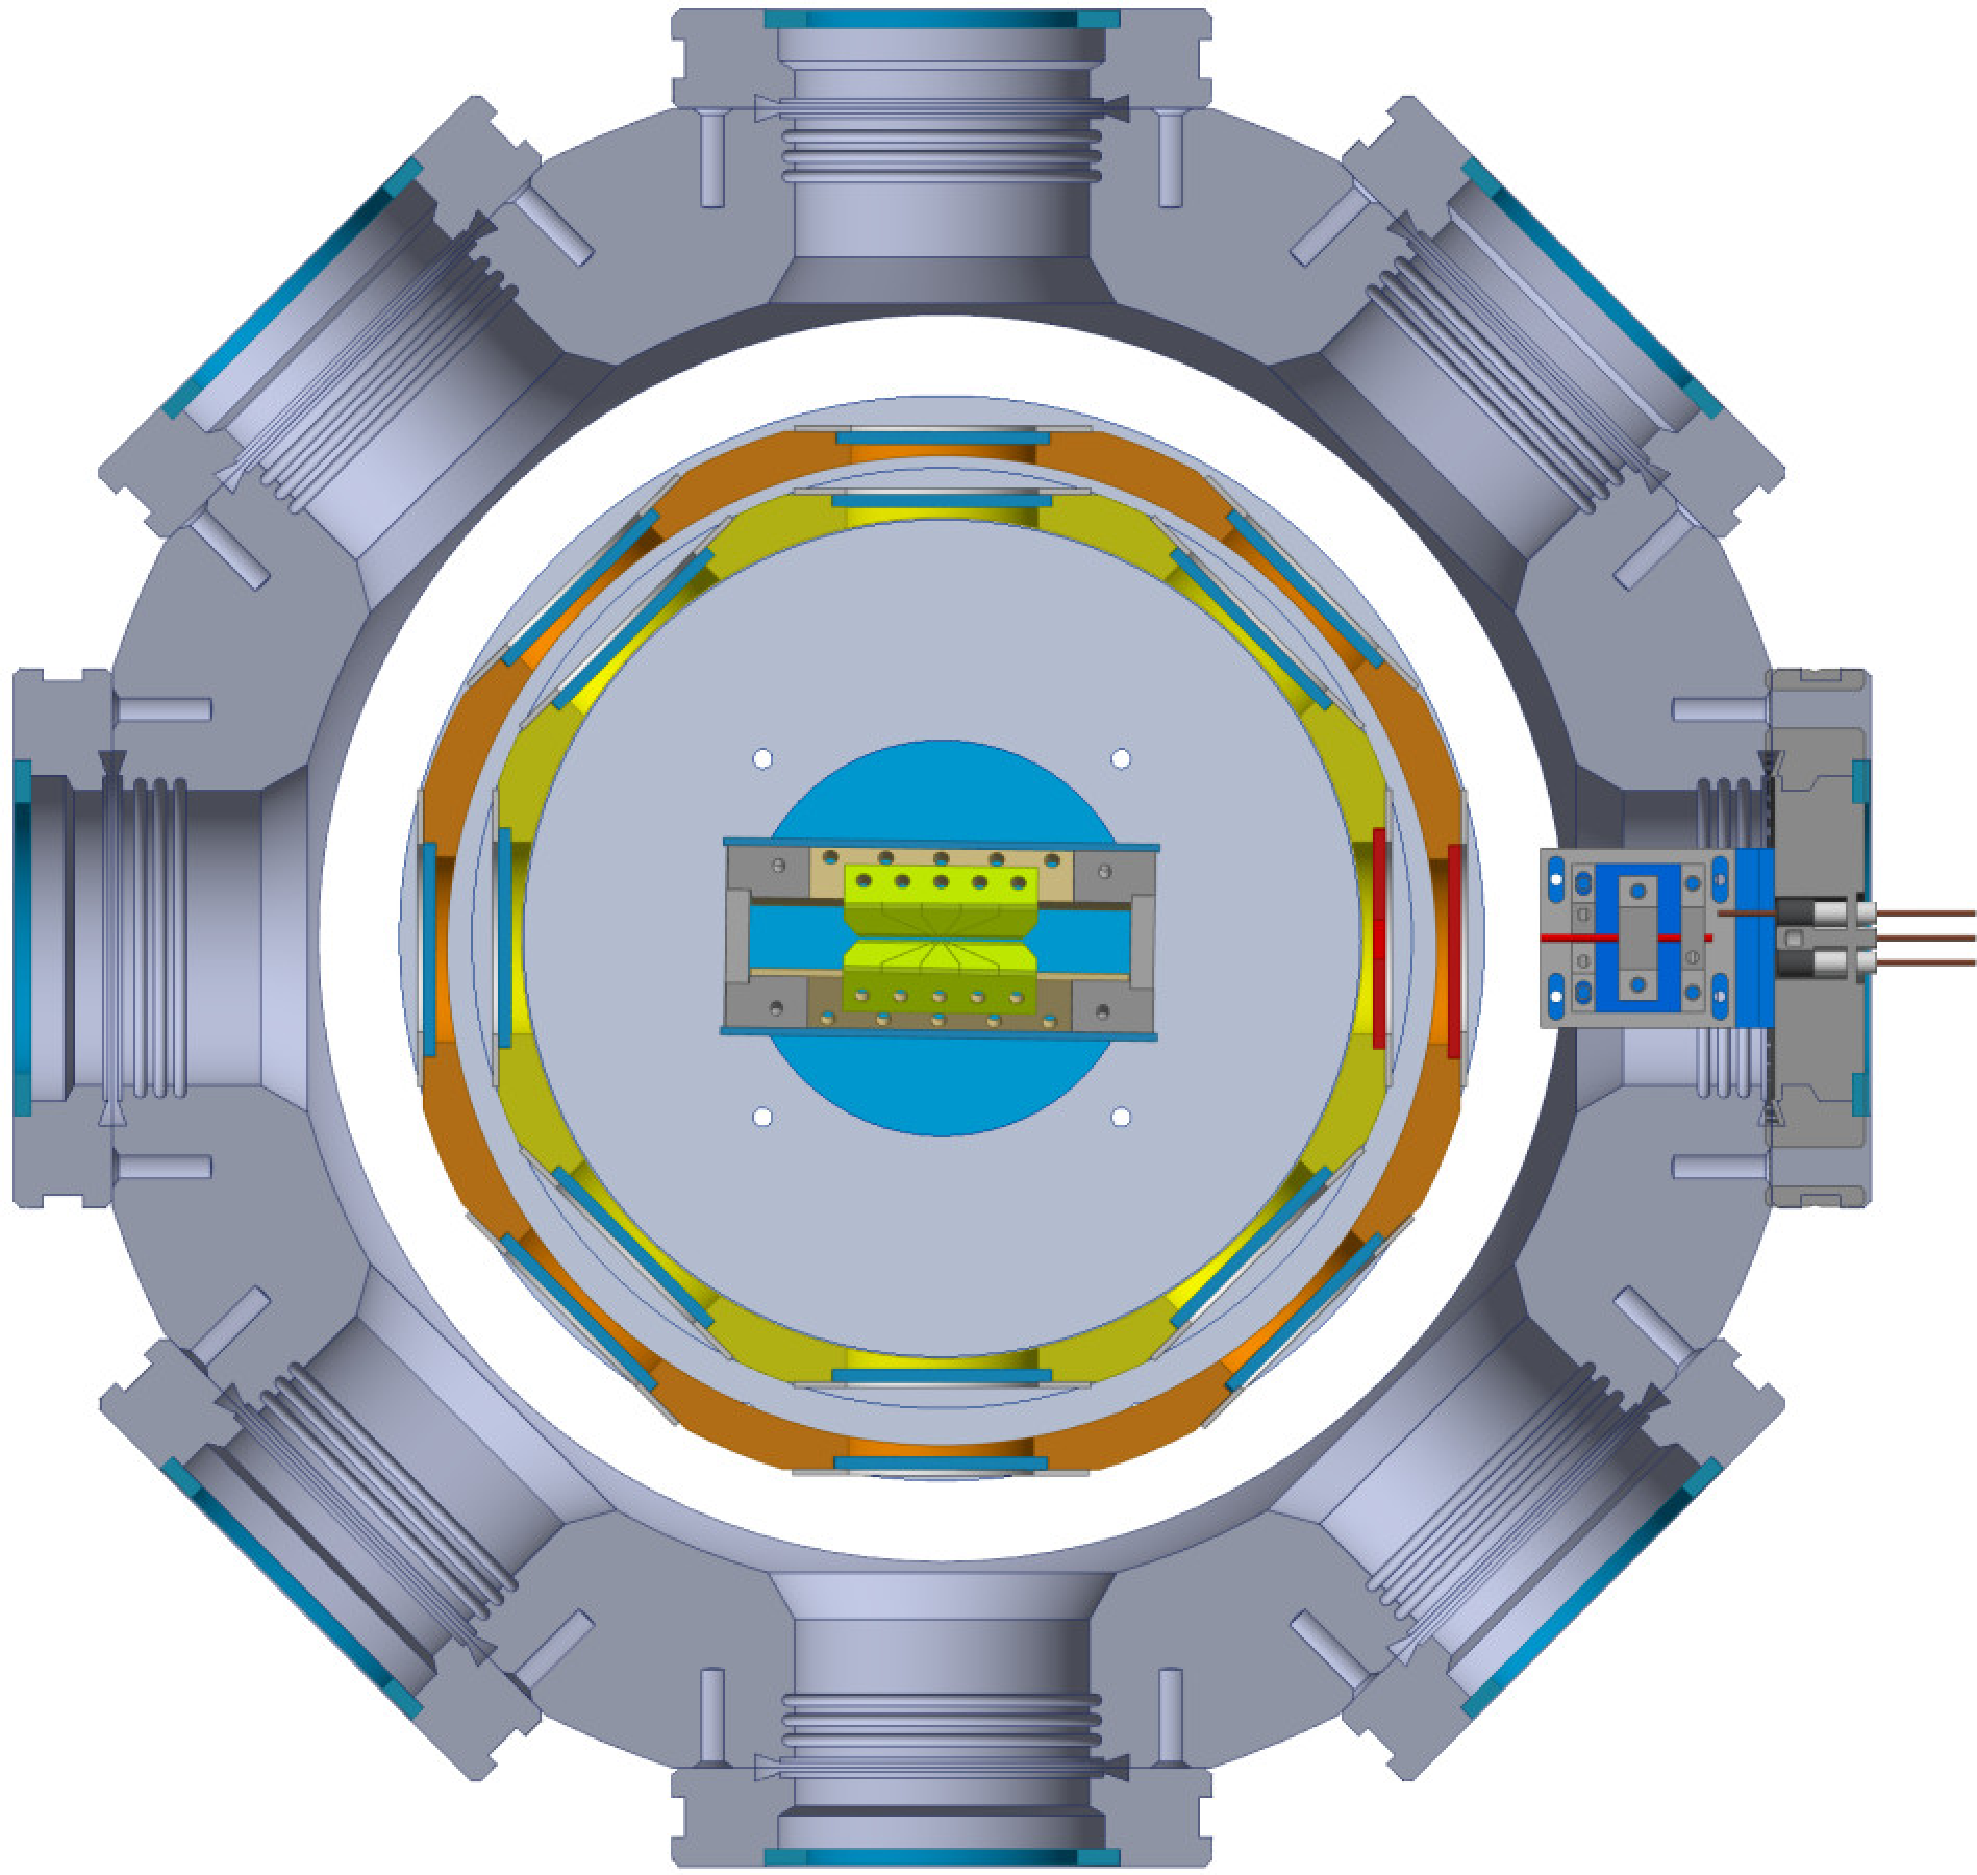
\includegraphics[width=0.4\linewidth]{fig_3_cryostat_c.pdf}}
    \caption{The design and related information of the cryostat.}
    \label{fig:cryostat}
\end{figure}

Although the refrigeration capacity of the 4 K stage in the cold head reaches 1.5 W, the cooling capacity of the sample mount in the vacuum chamber, which is directly available to the user, is much lower. The reduction of the cooling capacity comes from the heat conduction between the 4 K stage and the sample mount and the heat leakage from the environment. In order to improve the heat transfer between the 4 K stage and the sample mount, we can increase the surface area of the heat exchanger, we can also fill the exchange gas space with sufficient helium gas, and it is necessary to use oxygen-free copper to produce thermally conductive parts. In our experiments, we use auto gas charging system to stabilize the helium pressure in the exchange gas space at a fixed positive pressure. It is worth noting that the rubber bellow loses its vibration isolation function under negative pressure, and the life of the rubber bellow is reduced. The auto gas charging system was designed by PHYSIK and is based on the principle of using a PLC to read the helium pressure gauge and control the opening and closing moments of the helium valves, which will eventually stabilize the helium pressure gauge at 1.03 bar. There are two helium valves to control the helium inlet and outlet, and one safety value to allow excess helium to escape, preventing the bellow from bursting when the auto gas charging system is not working. The temperature stabilize system is a kit we purchased from Janis Inc. and consists of a thermometer, heater and temperature controller. The thermometer (DT-670-CU-HT-1.4H) is located inside the sample mount in the vacuum chamber and has a measurement range of 1.4-500 K, covering the cryostat operating range of approximately 4-300 K. The heater is a 25 Ohm resistor very close to the thermometer. The DC lines of the heater and the thermometer are connected to the temperature controller (Model 26 from CryoCon) on the instrument rack via a DC feedthrough on the vacuum chamber. In low temperature operation, the temperature of the sample mount can be stabilized at $6 \pm 0.05$ K for a long time by setting the appropriate PID parameters, as shown in Fig~\ref{fig:cryostat_temperature}. The output power of the heater is about 350 mW, which means that the refrigeration capacity of the sample mount has a margin of 350 mW.

\begin{figure}
    \centering
    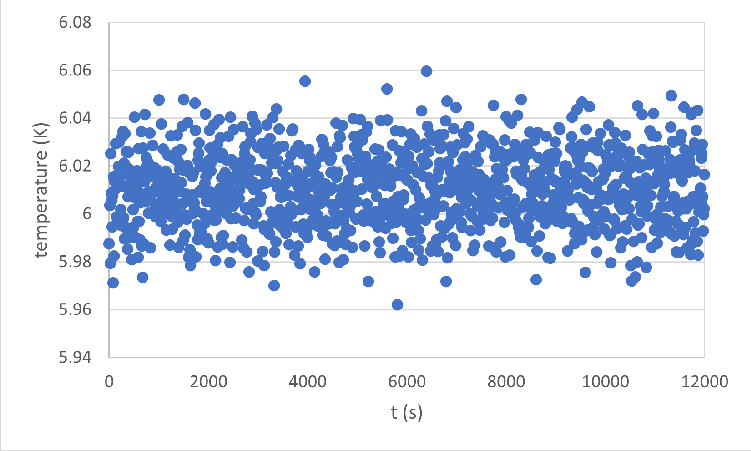
\includegraphics[width=0.7\linewidth]{fig_3_cryostat_temperature.pdf}
    \caption{The stablized temperature of the sample mount.}
    \label{fig:cryostat_temperature}
\end{figure}

The auto gas charging system and the temperature stabilize system are the key systems for the long-term stability of the cryostat. Although the temperature of This cryostat has almost no drift, we can observe that the trap can shift $\pm 1$ μm during the experiment. The operation to avoid the effects of such position shifts by frequent calibration of the system parameters is very complicated, so this instability can be fatal for an experimental system. The long drift of the sample mount comes from the mechanical structure of the cryostat. The auto gas charging system can only stabilize the helium pressure near the rubber bellow, and the 40 K stage and 4 K stage of the cold head are not stabilized. Therefore, the pressure and temperature in the contact part of the vacuum chamber and the exchange gas space cannot be stabilized for a long time. However, this part is the support point of the sample mount, so the sample mount will be disturbed by these external environmental changes. We can consider fixing the sample mount to the room temperature area of the vacuum chamber, which will not move if the laboratory environment is stable, but this will inevitably increase the heat leakage from the room temperature area. In our experiments, we first pumped the vacuum chamber to $1 \times {10}^{-6}$ mbar at room temperature using the Turbo Pump, then activated the NEG-Ion Pump for about 2 hours, and at the end of the operation the vacuum chamber vacuum level dropped to $1 \times {10}^{-8}$ mbar. The vacuum chamber can reach a vacuum level of $3 \times {10}^{-10}$ mbar with the effect of the cryo-pump.



\section{Helical resonator and segmented blade trap}

The blade trap forms a capacitor of approximately 6 pF. In order to drive this capacitor, i.e. to apply a high voltage signal to it, we need a larger helical resonator to form the LC oscillation circuit and to achieve impedance matching. The two components are therefore closely linked. The helical resonator and the blade trap are both located inside the 4 K shield of the vacuum chamber. The helical resonator is fixed underneath the sample mount and then the blade trap is fixed underneath the helical resonator. This ensures that the helical resonator and the blade trap are very close to each other and that their temperatures are equally stable. At the same time the low temperature allows the resistance in the oscillator circuit to be significantly reduced, which helps to increase the quality factor of the oscillator circuit. The helical resonator and the blade trap are used as a single unit and its input and output are achieved via RF and DC electric feedthrough.

\subsection{Design of helical resonator}

\begin{figure}
    \centering
    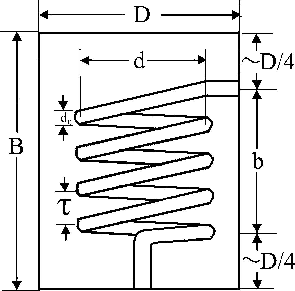
\includegraphics[width=0.5\linewidth]{fig_3_outline_design_of_a_helical_resonator.pdf}
    \caption{The outline design of a helical resonator.}
    \label{fig:outline_design_of_a_helical_resonator}
\end{figure}

The circuit models for the helical resonator and the blade trap have been well studied. In practice, we have developed a very mature design procedure with a high quality factor, choosing only two parameters $ b / d $ and $ d / D $ to optimise the performance of the helical resonator with the quality factor as the objective function. We can calculate the loading frequency in the empirical parameter regime using the trap capacitance and the quality factor. Typically, $ b / d \approx 1.5 $ and $ d / D \approx 0.5 $ is a good choice, and if the loading frequency meets our requirements we will try to choose the highest quality factor around this parameter range, as shown in Fig~\ref{fig:outline_design_of_a_helical_resonator}. A two-wire spiral resonator is much more complex than a single-wire spiral resonator because of the coupling between the two coils. However, for the sake of simplicity we are still using the model and we can achieve an accuracy of about $\pm 5$ MHz. To ensure that the phase and amplitude of the two coils are the same, we use a parallel capacitor, which is shorted when connected to the RF feedthrough, with a capacitance of approximately 300 nF. The two-wire design is designed to help minimise micro-movements by applying a DC voltage to the RF electrodes, so we need to ensure that the RF signal on the coil is grounded and the DC voltage is not, this is achieved by a 300 nF capacitor connected to the shield. In addition, we added an RC filter before the DC voltage was connected to the coil.

\subsection{Assembly of helical resonator}

The material used for the body of the helical resonator is oxygen-free copper, which is characterised by its very low resistivity and high thermal conductivity. The low resistivity helps to obtain a high quality factor, but the oxygen-free copper is susceptible to oxidation during processing, so the oxide film needs to be removed before assembly. After the helical resonator has been assembled, it needs to be placed in a vacuum enclosure to prevent oxidation.

The main parts of the helical resonator were machined according to the design parameters: the antenna cover, the top cover, the middle part, the bottom cover and the helical coils, which were then cleaned in the ultrasound machine using acetone and ethanol. After drying these parts with nitrogen and soaking them in organic acid for 5 minutes, it can be observed that the surface oxide film disappears and turns purplish red. We soak the parts in plenty of distilled water to remove the residual organic acid and then dry the parts with nitrogen. The cleaning of the parts of the main part of the copper tube is now complete. This part needs to be done carefully, as the oxide film on the helical resonator surface affects the quality factor.

We also need to prepare and clean the rest of the parts according to the design parameters to meet the ultra-high vacuum requirements. We then soldered the circuit components together using lead-free solder. The parts are then assembled with stainless steel screws, each requiring a resilient pad to prevent the screws from loosening at low temperatures.

\subsection{Assembly of blade trap}

The advantage of the blade trap is that it is easy to process and assemble, but the disadvantage is that the assembly error is higher compared to the surface trap or the monolithic trap, which causes an asymmetry in the electrostatic potential at the centre of the trap where the ions are located, i.e. a deviation from the linear trap configuration. When designing the blade trap for use in the cryostat, we need to take care that the material has a high thermal conductivity and that the connections between the components are sufficiently tight. In this way we can achieve the lowest temperatures on the blade trap. This helps to obtain a higher vacuum level and to extend the life of the ions.

The blade trap consists of four blade-shaped electrodes, one pair of DC electrodes and one pair of RF electrodes. The blade is processed by laser cutting the ceramic substrate and then plating the surface with a gold layer. The electrodes are machined with a certain amount of error and defects on the surface of the electrode closest to the ion produce a high level of electrical noise, which can be reduced by improving the process. We have machined a sapphire adapter plate and mounted the blade on the sapphire adapter plate and then mounted the sapphire adapter plate on an oxygen-free copper holder. We designed this adapter to avoid a short circuit between the blade and the ground (the blade holder). In order to increase the thermal conductivity, we need to cover these contact surfaces with indium foil. For the fixing of the components we used stainless steel screws and used resilient pads on each screw. This is to prevent the screws from loosening during the cooling down process, and to prevent the blade from being crushed by excessive torque when tightening the screws. Once installed we had to fine-tune the position of the sapphire adapter under the microscope to keep the assembly error small enough. This operation makes use of the fact that the diameter of the through-hole is slightly larger than the diameter of the screw. Since the assembly is done by hand, this part of the assembly error is unavoidable.

The connection of the blade electrodes is mainly done by means of gold ribbon (AMETEK) and Kapton insulated wire (Accu-Glass Products). When selecting materials we need to be aware of ultra-high vacuum and cryogenic compatibility. Some of the circuit connections are made prior to assembly and the rest is done afterwards. Before assembling the blade, a 820pF capacitor is fixed with silver epoxy between each DC electrode and ground on the two DC blades. The purpose of this capacitor is to create a low impedance between the DC electrodes and ground, reducing the voltage splitting of the RF signal on the DC electrodes. The gold ribbon is connected to the electrodes with the spot welder at one end and to the pads of the PCB with solder at the other. We will later connect the pads to the corresponding connections with Kapton insulated wire, where the DC electrode wires are connected to the corresponding wires from the DC feedthrough through the heat sink twice, and the two RF electrode wires are connected to the two wires at the output of the helical resonator.



\section{Yb oven}

In order to generate the atomic beams of Yb, we built two separate ovens from two stainless steel tubes, but integrated into a single feedthrough and both able to be used to load ions. The ${ }^{171} \mathrm{Yb}$ oven has an abundance of 90\% and The ${ }^{174} \mathrm{Yb}$ oven has an abundance of 98\%. As the Yb source is in block form, we need to cut it into small pieces and insert it into the stainless steel tube.

In order to achieve UHV compatibility we chose to use copper, stainless steel and Macor when machining the parts of the oven. Before assembly and testing, we cleaned all the parts inside the ultrasound machine using acetone and ethanol as solvents. All the parts were assembled according to the drawings and the copper wires on the feedthrough were attached to the stainless steel base, which was all screwed in place. We then used a spot welder and welded the stainless steel tube to the stainless steel wire, and the stainless steel wire to the stainless steel base, respectively. As the stainless steel tube has the smallest cross-sectional area, the highest resistance in the whole circuit is at the stainless steel tube, about 0.5 Ohm, so the temperature is highest here too. I would recommend having some extra spare parts and testing the parameters of the spot welder in advance, as the stainless steel tube can easily break under unsuitable parameters. Finally the two Yb sources are filled into the corresponding stainless steel tubes.

Each oven is mounted in such a way that the outgoing atomic beam is directed towards the trapping area. The oven feedthrough replaces an XX inch window in the axial direction of the trap. the glass in the corresponding position of the 40 K shield and 4 K shield is also replaced with a round aluminium plate, the centre of which is a square hole with a 5mm side to pass through the Yb flux. As the cryostat has assembly errors, I would recommend preparing round aluminium plates with different opening positions in advance. Ultimately we need to be able to see the trap through the opposite window, with the square hole and the oven in the same line.

In the process of loading ions, when this stainless steel tube is heated resistively by an electric current, a spray of atomic Yb is produced. The temperature reached depends on the current and the time of operation. If either of these two factors is too high or too long, this can lead to rapid evaporation of the Yb and thus the formation of a spray dense enough to cover its surface (e.g. ion trap electrodes or vacuum windows). To prevent this, each oven is tested in advance. A stainless steel sheet is placed in front of the oven and then the oven is placed in a transparent vacuum chamber and the vacuum is reduced to approximately 4E-6 mbar using a turbo-molecular pump, so that a test system can be set up. We tested each oven in turn, starting at 0 A and increasing the current by 0.1 A every 10 seconds, observing the change in vacuum level and the colour of the stainless steel sheet. We can observe both the darkening of the stainless steel sheet and the rapid rise in pressure, at which point the current value is the threshold current for the corresponding oven. ${ }^{171} \mathrm{Yb}$ oven has a threshold current of 4.2A and ${ }^{174} \mathrm{Yb}$ oven has a threshold current of 3.9A, but the current values we use in practice will be lower than this threshold, the exact values need to be measured in the corresponding experiments. The exact values need to be measured in corresponding experiments, such as observing the fluorescence of Yb atoms and loading Yb ion.



\section{Optical and imaging system}

Whether trapping ions or manipulating them, we need lasers. In our laboratory, tunable diode lasers (Toptica) are used widely, mainly because these products are very well mature. For ion trap systems, a stable light source is very important. Experimentally, we need these lasers to be switched on and off quickly, typically in a few hundred nanoseconds. It is also necessary that these lasers can be stabilised over long periods of time and that these laser controllers have stable software systems. Laser stabilisation covers mode, frequency, power and polarisation. Typical laser stabilisation lasts from a few hours to a day, including laser frequency locking. This is sufficient for our trapped ion experiments, but longer stabilisation times are preferable. In the experiments, these stable lasers are used for: ion loading, Doppler cooling, optical pumping, state detection, repumping and sympathetic cooling. In addition to the laser light path into the cavity, I also built an imaging system to collect the fluorescence emitted by the ions, enabling real-time observation and state detection of the ions.

\subsection{Laser sources and power allocation}

The light sources in the laboratory are placed on several separate optical tables. Since the principles of the optical path setup are similar, we can present the light sources and power allocation in a common way. The cryogenic trap platform requires a 370nm laser, a 399nm laser and two 935nm lasers. The two 935 nm lasers are shared with other ion trap platforms in the lab, one for trapping ${ }^{171} \mathrm{Yb}^{+}$ ions and the other for trapping ${ }^{174} \mathrm{Yb}^{+}$ ions. The 399nm laser is used for loading ions. Depending on the type of ion to be loaded, ${ }^{171} \mathrm{Yb}^{+}$ or ${ }^{174} \mathrm{Yb}^{+}$, we can change the wavelength of the 399nm laser. This 399nm laser is also shared with other trapped ion platforms in the lab and only one 399nm laser is needed. Since loading ions is not very frequent and most of the time we need to load ${ }^{171} \mathrm{Yb}^{+}$ ions, and modifying the wavelength of the 399nm laser will not affect the stable trapping of the loaded ions.

The output power of a semiconductor laser is approximately XXmW, depending on the wavelength and model, the laser output power may vary a little. The output power of the 370nm laser (L1) is XXmW, the output power of the 399nm laser (L2) is XXmW, the output power of the 935nm laser (L3) is XXmW and the output power of the 935nm laser (L4) is XXmW.

As the nominal light output from the laser is linearly polarised, a power attenuation unit was formed using a half-wave plate(HWP) and polarization beam splitter(PBS )to split the laser output into two parts, which are separately coupled into the fibre. Each fibre will act as the light source for the next stage of the optical path, thus making the optical path a modular one. Each laser has one optical fibre connected to the wavemeter (C5, C6, C7, C8). Because polarisation stabilisation is not required, a single-mode fibre is used, with a typical power of approximately 50 µW. The other fibres are the light sources for the rear optical paths (C1, C2, C3, C4) and require high power, typically 5 mW. At the same time their polarisation needs to be stable over time and we use single-mode polarization-maintaining fibres. In order to adjust the polarisation direction to match that of the single-mode polarisation-maintaining fibre, we use a polarisation adjustment unit consisting of a HWP and quarter-wave plate(QWP). We need to maximize the efficiency of the fiber coupling, which requires a good laser output mode and good mode matching, which can be done with a lens pair, I don't show this in the diagram.

The 370nm laser also has two splits: one (C9) is connected to the optical cavity for narrow linewidth frequency locking of the laser, and the other (C10) is set aside. ${ }^{171} \mathrm{Yb}^{+}$ repumping beam requires XX sidebands, so the 935nm laser (L3) has a fibre EOM (E1) in the rear optical path.

\subsection{Laser frequency stabilization}

The target linewidth of the laser frequency locking determines the laser frequency locking scheme. In my experiments there is no need for ultra-narrow linewidth laser locking, so the laser locking scheme is relatively simple and I have mainly optimised the automatic control of the frequency locking process. The measurement and locking of the laser frequency can be achieved with a wavelength meter, which has a relatively low bandwidth of about 10 Hz because the sum of the measurement time of the multi-channel wavelength meter and the computer readout time is about 100 ms. The standard deviation of the output frequency of the laser locked with this scheme is about 1MHz, which meets my needs with a 399nm laser and two 935nm lasers, or if only to trap a small amount of ions then also my requirements for a 370nm laser. The outgoing light from the laser is transmitted by optical fibres (C5, C6, C7, C8) to the input of the wavemeter, which is programmed to read the frequency on our PC and then programmed to adjust the voltage signal from the laser controller, thus creating a closed loop that locks the laser frequency. The wavemeter's measurements are affected by the environment, mainly air pressure and temperature. Therefore this frequency locking scheme will cause the locked laser frequency to be inaccurate due to inaccurate measurements, but this error is slow and periodic over time. So for 399nm laser and 935nm lasers we don't take this into account. I only calibrate the 370nm laser once in 1 hour or longer, by measuring the resonant frequency of the Yb+ ion and feeding it back to the wavemeter's lock point. It would be possible to automatically calibrate the wavemeter for measurement errors if the wavemeter had a locked reference light all the way through, such as a 780nm laser, but we have not done this because it is not necessary. The implementation of an automatic frequency lock is necessary as it will simplify the steps of daily operation. By laboratory standards these lasers need to be switched off when they are not in use, for example every night. I will adjust the operating parameters of the laser so that the laser mode can be stabilised back to a specific frequency range for approximately 10 minutes after each switch-on operation, which requires us to find a stable operating parameter for the laser. We then only need to program to communicate with the laser and the wavemeter to achieve automatic laser control and frequency locking.

The results of targeting the 370nm laser with a wavemeter are not good enough because the feedback speed is too slow. We can increase the feedback speed with the assistance of an optical cavity, which reduces the standard deviation of the output frequency of the 370 nm laser to 300 kHz. I built this optical path on a breadboard in which an optical cavity (U2; SA200-3B, Thorlabs) was placed. The outgoing light from the 370 nm laser (C9) is incident to the optical cavity. mode matching of the optical cavity is achieved by a pair of reflectors and lenses. Locking the 370nm laser to the optical cavity is achieved by feeding the output signal of the photodiode (D1) back to the voltage signal of the 370nm laser controller. In order to have the lock point at the point of maximum transmission light intensity of the optical cavity, I added a modulation signal to the current signal of the 370nm laser and demodulated the signal from the photodiode (D1). This solution uses a simple optical cavity to increase the bandwidth of the laser locking. This scheme uses a simple optical cavity to increase the bandwidth of the laser locking. However, because environmental factors can cause the cavity length of the optical cavity to change, the locked frequency will change rapidly as the cavity length changes. I connected the voltage signal (S1) from the wavemeter output to the piezoelectric ceramic (P1) of the optical cavity, thus achieving a locking of the optical cavity length to the wavemeter.

\subsection{Laser modulation}

Making the laser modulation a separate module allows for modularisation of the optical path, which facilitates maintenance and testing, and also reduces the size of the optical path into the cavity, which in turn reduces the area of the breadboard where the cryogenic trap vacuum chamber is located. The main source of laser leakage during laser modulation is the higher order modes of the laser and stray light from the crystal during modulation. Adding a stage of fibre coupling can act as a spatial filter and help reduce leakage.

Experimentally, I need to add sidebands to the 370nm laser, the 14.7GHz sideband (E2) for Doppler cooling and the 2.105GHz sideband (E3) for optical pumping. the electro-optic modulator(EOM) can implement these features. The frequency and modulation depth of the sidebands can be controlled by controlling the frequency and amplitude of the EOM input microwave signal. In addition, I need to control the frequency shift and power of the 370nm laser. This is because the difference in frequency required for Doppler cooling and state detection is approximately 12MHz, and the frequency variation measured during calibration of the system can be compensated for by adjusting the frequency shift of the 370nm laser. The acousto-optic modulator(AOM) provides these features. By controlling the frequency and amplitude of the microwave signal input to the AOM(A1) the frequency of the laser shift and the laser power can be controlled.

The light source from the 370nm laser is fed to the laser modulation module via a single-mode polarization-maintaining fibre (C1), which is reflected by a beam sampling mirror and enters the laser monitoring module (U3). A number of signal acquisition modules are integrated into the laser monitoring module to help me monitor the quality of the light source over time, including measurements of power , polarisation, laser mode and others. The main light source is modulated by two cascaded EOMs, the modulation depth of which can be maximised by adjusting the HWP. Part of the laser is coupled into the fibre (C12), which is then used for sympathetic cooling. To achieve the frequency shift, I built a double-pass configuration based on a 4f optical system, where the PBS serves to separate the incident light from the returned light by 90°, adjusting the HWP at the front to maximise the efficiency of the incident light and the HWP at the back to maximise the efficiency of the diffraction from the AOM. When the laser passes through the AOM, 0 order light is discarded and +1 order light is returned to the AOM by a 4f optical system consisting of a lens and a D-shaped pickoff mirror. The +1 order beam from the reflected beam passes through the QWP twice and is then reflected by the PBS into the fibre (C11), this light is then used for global cooling, pumping and detection. There is a mechanical shutter(N1) in front of the fibre, which serves to completely shut off the light and reduce leakage.

\subsection{Optical layout of cryostat breadboard}

Due to the large base area of the cryostat, the area left for the optical path on the breadboard is relatively small. the main function of the optical path built on the breadboard of the cryostat is to shape the beam into a specific shape and then inject it into the cavity. There are four windows on the Cryostat that are used to inject the laser. The laser light exiting the fibre collimator (C2, C3, C4, C11, C12) is first polarised by the QWP and HWP and then expanded by the lens pairs (T1, T2, T3, T4) to a suitable spot size, typically with a Gaussian diameter of approximately 10 mm. It is then incident on a long-focus lens (L1, L3, L5, L7) into the cavity and forms a small spot in the centre of the trap, typically with a Gaussian diameter of about 20 μm. The long-focus lenses are mounted on a 3-axis linear stage (G1, G2, G3, G4; M-461-XYZ-M, Newport) with a Picomotor actuator (8301NF, Newport) in each axis of the stage to achieve high precision control of the beam position. Reducing the spot diameter at the trap is necessary to increase the power density, reduce stray light and improve the signal to noise ratio. It also helps me to monitor the displacement of the spot relative to the ions over time, which helps me to find unstable components or modules in the system at the beginning of the construction of the system. But when the length of the ion chain in the trap increases, I need some light spots to expand in the horizontal direction to about 500 μm in diameter. It is advantageous to be able to easily adjust the spot diameter in the horizontal direction. I added cylindrical lenses (L2, L4, L6) to the optical path where I needed to adjust the horizontal diameter, and by artificially introducing astigmatism, I was able to shift the horizontal focal position along the optical axis. A long-focused cylindrical lens with a focal length of approximately 1000 mm is generally used, mounted on a rotatable lens mount so that the tilt angle of the elliptical spot can be adjusted and the cylindrical lens can be removed when the elliptical spot is not required.

The stability of the 370nm laser (C11) is so important to the experiment that a laser monitoring module (U4) has been installed at the outgoing point of the fiber. This light is global light and is required for ion loading, Doppler cooling, optical pumping, and state detection. In order to trap both ${ }^{171} \mathrm{Yb}^{+}$ and ${ }^{174} \mathrm{Yb}^{+}$, two 935nm lasers (C3 and C4) were combined into the cavity and their function was rupumping. Combining these two 935nm lasers at the front stage would have been a better option, but this was not done due to space planning in the laboratory. The 399nm laser (C2) is used for ion loading and the 370nm laser (C12) is used for sympathetic cooling.

A permanent magnet is placed in front of one window to generate a magnetic field at the centre of the trap, approximately XX Gauss, perpendicular to the direction of the ion chain. A horn is placed in front of one of the windows to apply microwaves.
